\documentclass[a4paper,14pt]{article} % тип документа
%\documentclass[14pt]{extreport}
\usepackage{extsizes} % Возможность сделать 14-й шрифт


\usepackage{geometry} % Простой способ задавать поля
\geometry{top=20mm}
\geometry{bottom=25mm}
\geometry{left=15mm}
\geometry{right=15mm}

\setcounter{section}{0}

%%%Библиотеки
%\usepackage[warn]{mathtext}
%\usepackage[T2A]{fontenc} % кодировка
\usepackage[utf8]{inputenc} % кодировка исходного текста
\usepackage[english,russian]{babel} % локализация и переносы
\usepackage{caption}
\usepackage{listings}
\usepackage{amsmath,amsfonts,amssymb,amsthm,mathtools}
\usepackage{wasysym}
\usepackage{graphicx}%Вставка картинок правильная
\usepackage{float}%"Плавающие" картинки
\usepackage{wrapfig}%Обтекание фигур (таблиц, картинок и прочего)
\usepackage{fancyhdr} %загрузим пакет
\usepackage{lscape}
\usepackage{xcolor}
\usepackage{dsfont}
%\usepackage{indentfirst}
\usepackage[normalem]{ulem}
\usepackage{hyperref}




%%% DRAGON STUFF
\usepackage{scalerel}
\usepackage{mathtools}

\DeclareMathOperator*{\myint}{\ThisStyle{\rotatebox{25}{$\SavedStyle\!\int\!\!\!$}}}

\DeclareMathOperator*{\myoint}{\ThisStyle{\rotatebox{25}{$\SavedStyle\!\oint\!\!\!$}}}

\usepackage{scalerel}
\usepackage{graphicx}
%%% END 

%%%Конец библиотек

\newcommand{\drawsome}[1]{            % Для быстрой вставки картинок
    \begin{figure}[h!]
            \centering
            \includegraphics[scale=0.7]{#1}
            \label{fig:first}
    \end{figure}
}
\newcommand{\drawsomemedium}[1]{
    \begin{figure}[h!]
            \centering
            \includegraphics[scale=0.45]{#1}
            \label{fig:first}
    \end{figure}
}
\newcommand{\drawsomesmall}[1]{
    \begin{figure}[h!]
            \centering
            \includegraphics[scale=0.3]{#1}
            \label{fig:first}
    \end{figure}
}

%%%Настройка ссылок
\hypersetup
{
colorlinks=true,
linkcolor=blue,
filecolor=magenta,
urlcolor=blue
}
%%%Конец настройки ссылок


%%%Настройка колонтитулы
	\pagestyle{fancy}
	\fancyhead{}
	\fancyhead[L]{Домашнее задание}
	\fancyhead[R]{Крейнин Матвей, группа Б05--005}
	\fancyfoot{}
    \fancyfoot[C]{\thepage}
    \fancyfoot[R]{ТРЯП}
%%%конец настройки колонтитулы


\begin{document}
%%%%Начало документа%%%%

\section{Задание 7}
\subsection{Задача 1}
Построим суффиксный автомат $\mathcal{A}$ по алгоритму, вот разные его стадии.

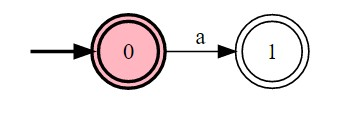
\includegraphics{01.jpg}

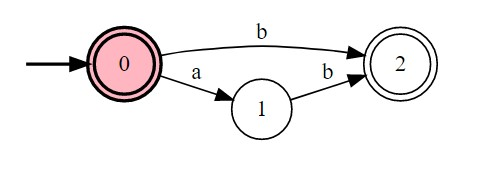
\includegraphics{02.jpg}

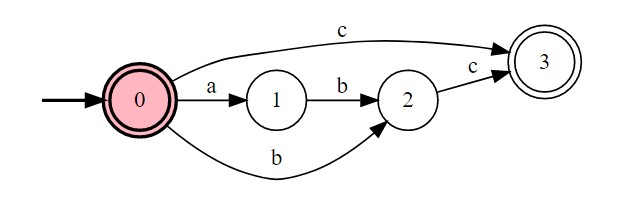
\includegraphics{03.jpg}

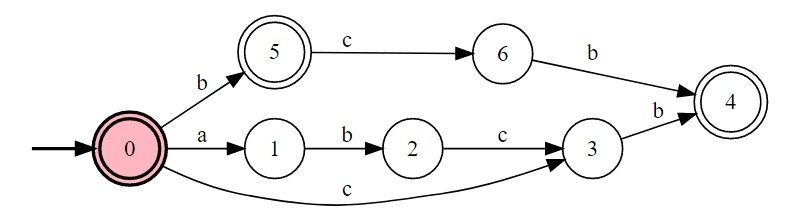
\includegraphics{04.jpg}

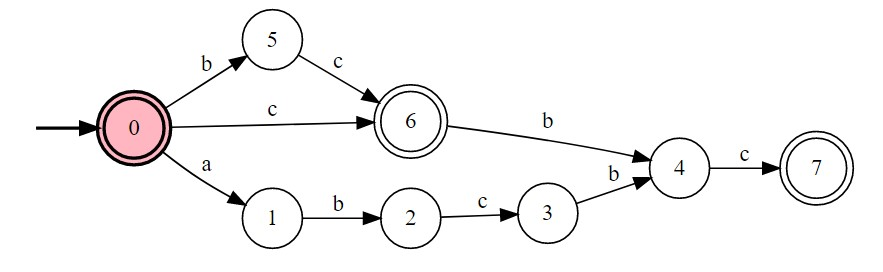
\includegraphics{05.jpg}

\textbf{1.} Минимальное количество раз, если только будет встречаться в подсловах bcbc по одному разу и ни в каких других больше, получится 20 раз.
Максимальное количество раз, если припишем к каждому bcbc по c в начале, получим 40 раз, и припишем к оставшемся 20 bc c в начало, получим еще 20 раз. Итого максимум получится 60 раз.

\underline{Ответ:} от 20 до 60 раз включительно.
\newline
\textbf{2.} Т.к. $\epsilon \in Suff(abcbc)$, то получается, что это вообще любое слово, но будем считать, что это не так.
\newline
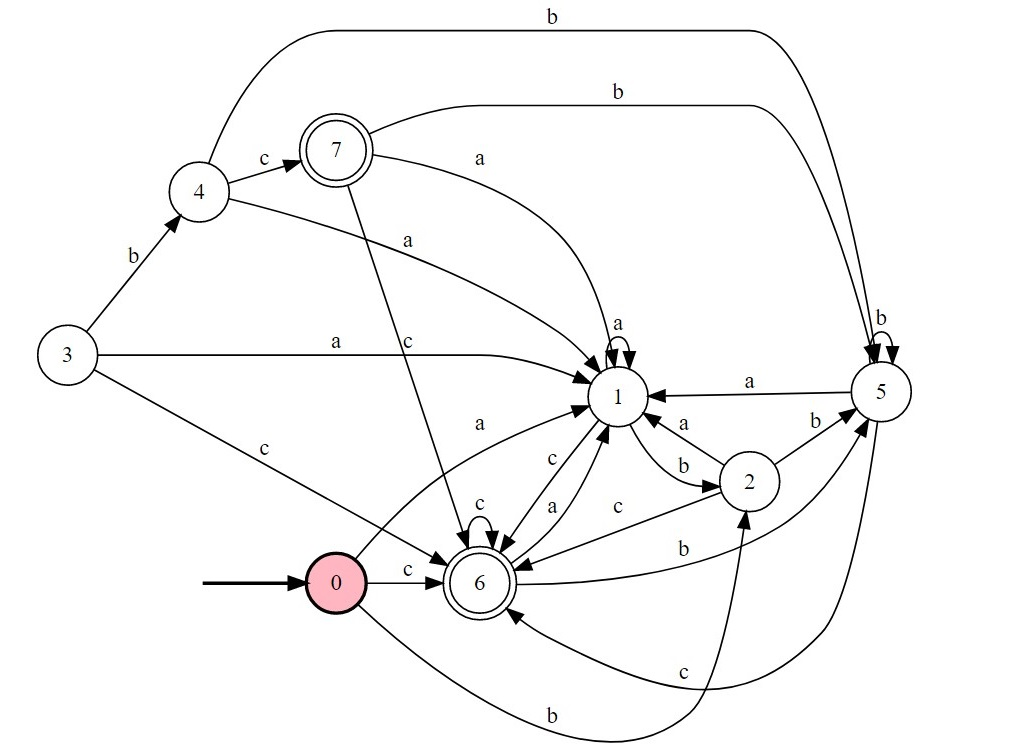
\includegraphics[scale=0.95]{06.jpg}

Но вообще, это всё что угодно, что заканчивается на c, поэтому ДКА выглядит вот так:

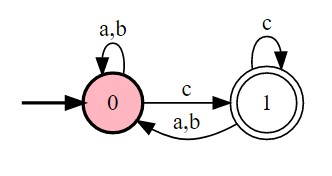
\includegraphics{07.jpg}

\textbf{3.} Coming soon...

%\subsection{Задача 2}
%\textbf{1.} X = ((110)* +111*)X.
%\newline
%\textbf{а) 111} \textbf{б) $((110)^*|111^*)^*$} \textbf{в) $((110)^*|111^*)^*$}
%\newline
%\textbf{2.} X = (00 + 01 + 10 + 11)X + (0 + 1 + $\varepsilon$)
%\newline
%\textbf{а) 0} 
%\textbf{б) $(00|01|10|11)^*(0|1|\varepsilon)$} 
%\textbf{в) $(\Sigma \Sigma)^*(0|1|\varepsilon)$ $=$ $\Sigma^*$}
%\newline
%\textbf{3.} 
%\begin{equation*}
%     \begin{cases}
%       \text{$Q_0$ = 0$Q_0$ + 1$Q_1$ + $\varepsilon$}\\
%       \text{$Q_1$ = 1$Q_0$ + 0$Q_2$}               \\
%       \text{$Q_2$ = 0$Q_0$ + 1$Q_2$}
%     \end{cases}
%\end{equation*}
%
%\begin{equation*}
%    \begin{cases}
%      \text{$Q_0$ = $0^*(1Q_1$ + $\varepsilon$)}\\
%      \text{$Q_1$ = 1$Q_0$ + 0$Q_2$}               \\
%      \text{$Q_2$ = 0$Q_0$ + 1$Q_2$}
%    \end{cases}
%\end{equation*}
%
%\begin{equation*}
%    \begin{cases}
%      \text{$Q_0$ = $0^*(1Q_1$ + $\varepsilon$)}\\
%      \text{$Q_1$ = $(10^*1)^*(10^* + 0Q_2$}  \\
%      \text{$Q_2$ = 0$Q_0$ + 1$Q_2$}
%    \end{cases}
%\end{equation*}
%
%\begin{equation*}
%  \begin{cases}
%    \text{$Q_0$ = $0^*(1Q_1$ + $\varepsilon$)}\\
%    \text{$Q_1$ = $(10^*1)^*(10^* + 0Q_2$}  \\
%    \text{$Q_2$ = $(0(10^*1)^*0 + 1)Q_2 + 0(10^*1)^*10^*1$}
%  \end{cases}
%\end{equation*}
%
%\begin{equation*}
%  \begin{cases}
%    \text{$Q_0$ = $0^*(1Q_1$ + $\varepsilon$)}\\
%    \text{$Q_1$ = $(10^*1)^*(10^* + 0Q_2$}  \\
%    \text{$Q_2$ = $(0(10^*1)^*0 + 1)^*0(10^*1)^*10^*1$}
%  \end{cases}
%\end{equation*}
%
%\begin{equation*}
%  \begin{cases}
%    \text{$Q_0$ = $0^*(1(10^*1)^*(10^*|0(0(10^*1)^*0|1)^*0(10^*1)^*10^*1 | \varepsilon$)}\\
%    \text{$Q_1$ = $(10^*1)^*(10^*|0(0(10^*1)^*0|1)^*0(10^*1)^*10^*1$}  \\
%    \text{$Q_2$ = $(0(10^*1)^*0|1)^*0(10^*1)^*10^*1$}
%  \end{cases}
%\end{equation*}
%\newline
%\textbf{а) частное решение} $Q_0 = 0, Q_1 = 011, Q_2 = 011$
%\newline
%\textbf{б) решение, минимальное по включению}
%\newline
%\textbf{в)}
%\begin{equation*}
%  \begin{cases}
%    \text{$Q_0$ = $0^*(1(10^*1)^*(10^*|0(0(10^*1)^*0|1)^*0(10^*1)^*10^*1 | \varepsilon$)}\\
%    \text{$Q_1$ = $(10^*1)^*(10^*|0(0(10^*1)^*0|1)^*0(10^*1)^*10^*1$}  \\
%    \text{$Q_2$ = $(0(10^*1)^*0|1)^*0(10^*1)^*10^*1$}
%  \end{cases}
%\end{equation*}
%
%\subsection{Задача 3}
%Автомат из диаграммы:
%\newline
%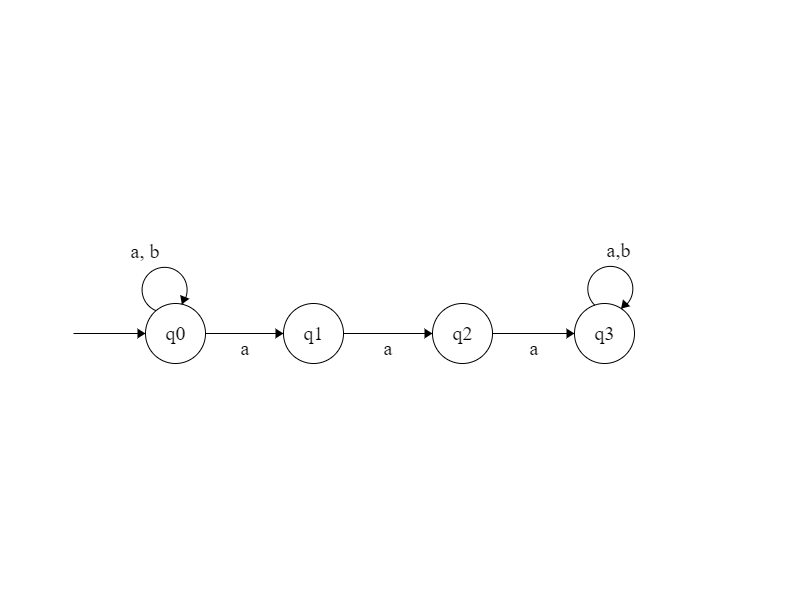
\includegraphics[scale=0.6]{08.png}
%
%Запишем систему для того, чтобы определить регулярное выражение для языка, который порождает этот автомат.
%\newline
%\begin{equation*}
%  \begin{cases}
%    \text{$R_{q0} = aR_{q0} + bR_{q0}+aR_{q1}$}\\
%    \text{$R_{q1} = aR_{q2}$}  \\
%    \text{$R_{q2} = aR_{q3} $} \\
%    \text{$R_{q3} = aR_{q3} + bR_{q3} + \varepsilon$} \\
%  \end{cases}
%\end{equation*}
%\newline
%Решаем её и получаем:
%\begin{equation*}
%  \begin{cases}
%    \text{$R_{q0} = (a|b)^*aaa(a|b)^*$}\\
%    \text{$R_{q1} = aa(a|b)^*$}  \\
%    \text{$R_{q2} = a(a|b)^*$} \\
%    \text{$R_{q3} = (a|b)^*$} \\
%  \end{cases}
%\end{equation*}
%
%Строим автомат по правилу построения НКА по РВ, упустим очевидные шаги этого построения и предоставим ответ (там реально много рисовать надо):
%\newline
%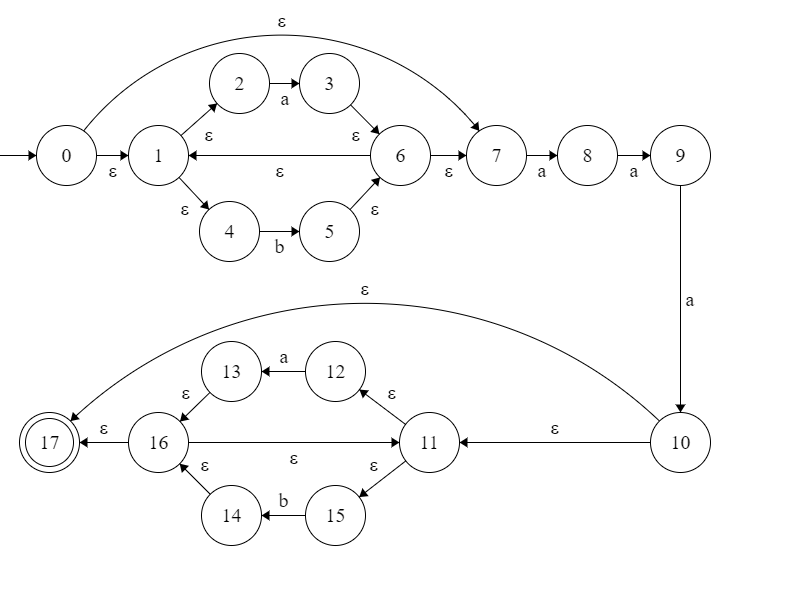
\includegraphics[scale=0.75]{09.png}
%\newpage
%Таблица переводов НКА в ДКА для $\mathcal{A}_2$:
%\newline
%\begin{tabular}{|l|l|l|l|}
%  \hline
%        &                                & a     & b    \\ \hline
%  $->Q_0$  & 0, 1, 2, 4, 7                  & $Q_1$  & $Q_2$ \\ \hline
%  $Q_1$  & 3, 6, 7, 8                     & $Q_3$  & --  \\ \hline
%  $Q_2$  & 1, 2, 4, 5, 6, 7               & $Q_4$  & $Q_2$ \\ \hline
%  $Q_3$  & 8, 9                           & $Q_5$  & --  \\ \hline
%  $Q_4$  & 1, 2, 3, 4, 6, 7, 8            & $Q_6$  & $Q_2$ \\ \hline
%  $Q_5$  & 9, 10, 11, 12, 14              & $Q_7$  & $Q_8$ \\ \hline
%  $Q_6$  & 1, 2, 3, 4, 6, 7, 8, 9         & $Q_9$  & $Q_2$ \\ \hline
%  $Q_7^*$  & 10, 11, 12, 13, 14, 16, 17     & $Q_1$0 & $Q_8$ \\ \hline
%  $Q_8^*$  & 11, 12, 14, 15, 16, 17         & $Q_1$0 & $Q_8$ \\ \hline
%  $Q_9$  & 1, 2, 3, 4, 6, 7, 8, 9, 10     & $Q_1$1 & $Q_2$ \\ \hline
%  $Q_{10}^*$ & 11, 12, 13, 14, 16, 17         & $Q_1$0 & $Q_8$ \\ \hline
%  $Q_{11}^*$ & 1, 2, 3, 4, 6, 7, 8, 9, 10, 17 & $Q_1$2 & $Q_2$ \\ \hline
%  $Q_{12}$ & 3, 8, 9, 10                    & $Q_1$3 & --  \\ \hline
%  $Q_{13}$ & 9, 10                          & $Q_1$4 & -- \\ \hline
%  $Q_{14}$ & 10, 11, 12, 14                 & $Q_1$0 & $Q_8$ \\ \hline
%  \end{tabular}
%\newline
%\newline
%Теперь таблица переводов из НКА в ДКА для $\mathcal{A}_1:$
%\newline
%  \begin{tabular}{|l|l|l|l|}
%    \hline
%     &            & a    & b    \\ \hline
%    $Q_0$  & 0          & $Q_1$ & $Q_0$ \\ \hline
%    $Q_1$  & 0, 1       & $Q_2$ & $Q_0$ \\ \hline
%    $Q_2$  & 0, 1, 2    & $Q_3$ & $Q_0$ \\ \hline
%    $Q_3$  & 0, 1, 2, 3 & $Q_3$ & $Q_4$ \\ \hline
%    $Q_4$  & 0, 3       & $Q_5$ & $Q_4$ \\ \hline
%    $Q_5$  & 0, 1, 3    & $Q_3$ & $Q_4$ \\ \hline
%    \end{tabular}
%\newline
%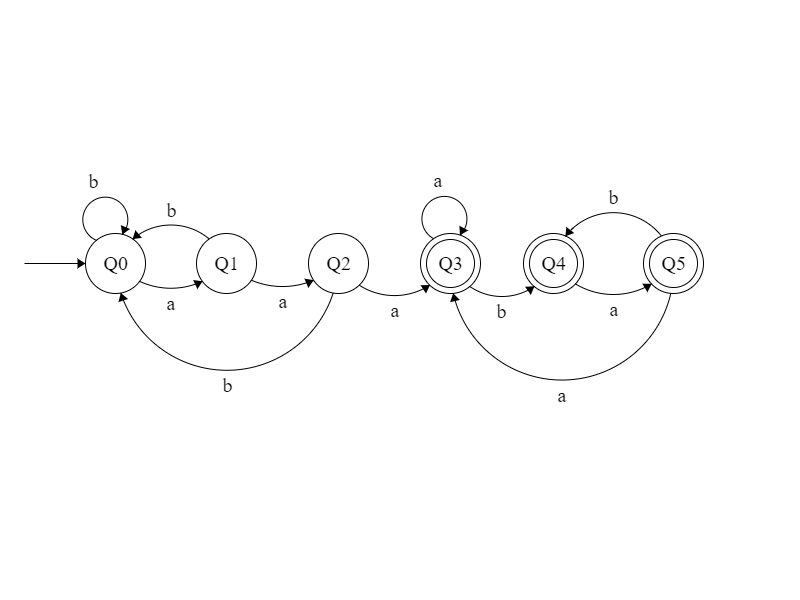
\includegraphics[scale=0.45]{10.png}
%\newline
%Построим таблицу followpos-ов для полученного регулярного выражения:
%\newline
%По таблице построим автомат $\mathcal{D}_2$:
%\newline
%\begin{tabular}{|l|l|}
%  \hline
%  i    & followpos(i)     \\ \hline
%  $1_a$ & $1_a, 2_b, 3_a$ \\ \hline
%  $2_b$ & $1_a, 2_b, 3_a$ \\ \hline
%  $3_a$ & $4_a          $ \\ \hline
%  $4_a$ & $5_a          $ \\ \hline
%  $5_a$ & $6_a, 7_b, 8  $ \\ \hline
%  $6_a$ & $6_a, 7_b, 8  $ \\ \hline
%  $7_b$ & $6_a, 7_b, 8  $ \\ \hline
%  \end{tabular}
%\newline
%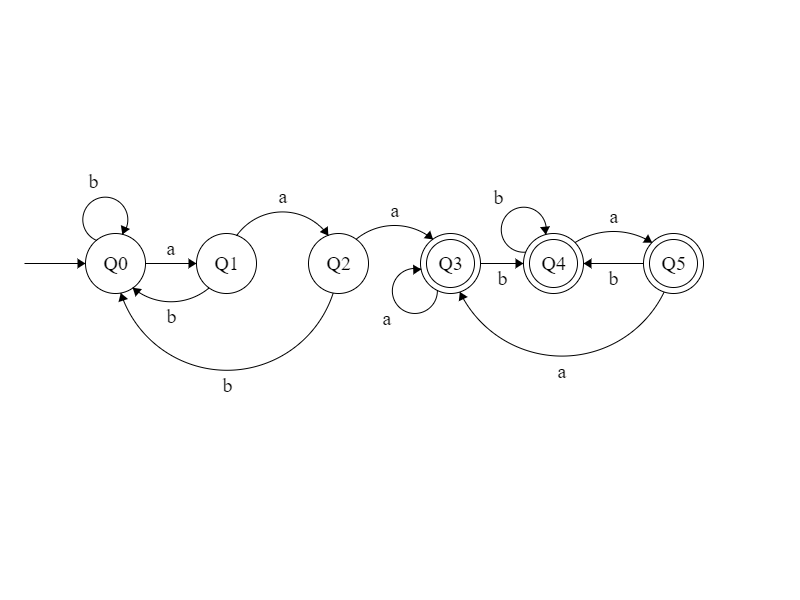
\includegraphics[scale=0.55]{12.png}
%\newline
%Теперь минимизируем данный автомат:
%\newline
%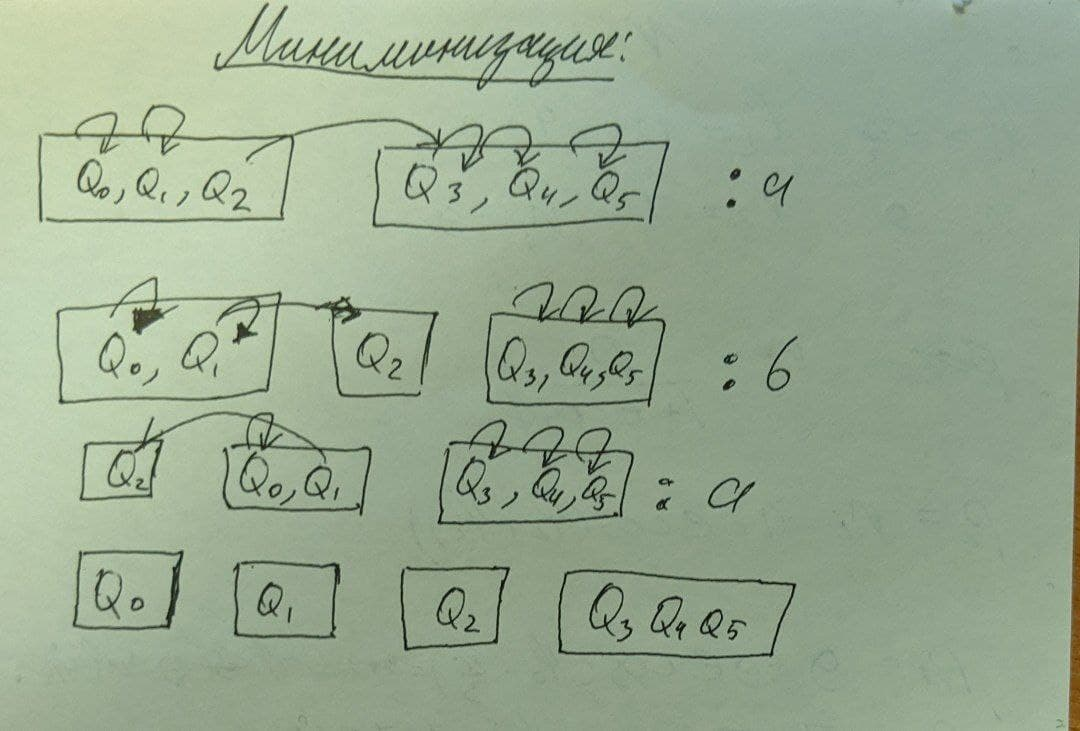
\includegraphics[scale=0.2]{13.jpg}
%\newline
%Построим ДКА по минимизарованному автомату:
%\newline
%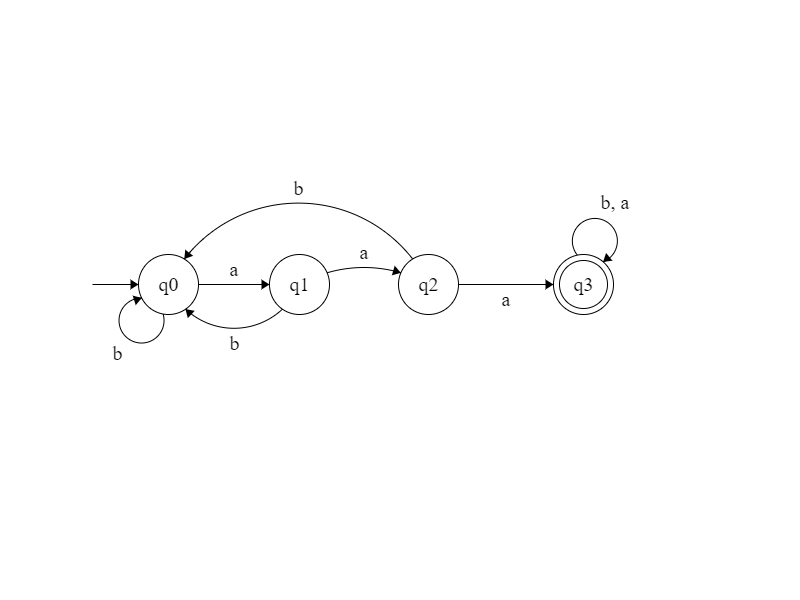
\includegraphics[scale=0.65]{14.png}
%\newline
%Теперь еще можем построить КПМ автомат с суффиксными ссылками:
%\newline
%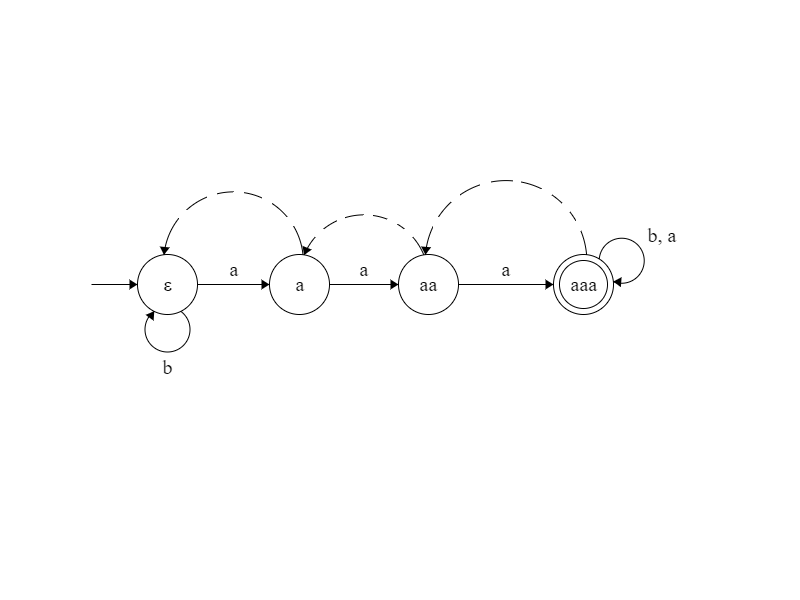
\includegraphics[scale=0.95]{15.png}
\end{document}